% !TeX root = ../../main.tex

\chapter{Testfälle}

In diesem Abschnitt wird die entwickelte Applikation in drei Testfällen getestet.
Die Testfälle sind dabei verschiedene Szenen mit mehreren Bildern von einem Objekt, das rekonstruiert werden soll.
Die Szenen und die Objekte sind dabei so gewählt, dass sie möglichst unterschiedlich sind in Bezug auf Größe und Beschaffenheit des Objekts.
In jedem Testfall wird die Szene kurz beschrieben und die Qualität der Feature Matches, sowie ihre rekonstruierten Punkte bewertet.
Bei der Bewertung wird zu einem auf die Beschaffenheit der Szene und des Objekts und zum anderem auf die Implementierung eingegangen.
In XXX werden die Ergebnisse der Testfälle zusammengefasst.

\section{Fall 1: Sessel}
Im ersten Testfall wird versucht einen Sessel zu rekonstruieren.
Dazu werden 10 Bilder verwendet, welche den Sessel aus verschiedenen Winkeln zeigt.
Die Bilder sind so sortiert, dass die Bewegung zwischen zwei Bildern minimal ist.
Die Anzahl der Matches, der rekonstruierten Punkte, sowie die Anzahl der Weltpunkte, die für die Skalierung genutzt wurden, so wie Skalierung selbst werden in \cref{tab:chair-results} gezeigt. % TODO: rewording
Das erste Bildpaar des Sessels wird in \cref{fig:chair-first-pair} gezeigt.
In \cref{fig:chair-first-pair-with-matches} wird das selbe Bildpaar mit allen Keypoints und ihren Matches gezeigt.
Matches sind dabei durch Linien gekennzeichnet, die die korrespondierenden Bildpunkte miteinander verbinden.
Hier fällt auf, dass sich die Matches überwiegend auf den Seiten des Sessels befinden.
Auch der Text auf der Decke und dem Kissen, so wie das karierte Muster des anderen Kissens werden als Keypoints erkannt und gematcht. % todo: rewording.
Des Weiteren sind viele Keypoints und Matches auf dem Teppich unten im Bild zu erkennen.
Im Gegensatz dazu gibt es sehr wenige Matches auf dem Boden, der Heizung, der Wand, sowie auf der Decke und dem Sitzkissen des Sessels.
Dies liegt daran, dass diese Texturen keine Kanten besitzen, die von den Feature Extractor als Feature erkannt werden können.
Dementsprechend fehlen diese Flächen bei den rekonstruierten Punkten, wie in \cref{fig:chair-model} zu sehen ist.  
Die generelle Form des Sessels und der Kissen ist in dem Modell gut zu erkennen.
Von der Decke ist nur ein streifen zu sehen, wo Matches an dem Text existieren.  
Das Sitzkissen ist überhaupt nicht zu sehen.
In \cref{fig:chair_model_2} ist das Modell von der anderen Seite und einem höheren Blickwinkel zu sehen.
Hier sind mehrere Punktsammlungen zusehen, die das gleiche darstellen, aber verschoben sind.
So etwa die Vorderseite und die Kissen des Sessels.
Dies lässt eine ungenaue Skalierung des Translationsvektors vermuten.

\begin{table}
    \begin{tabularx}{\textwidth}{c r r r r}
        \toprule
        Bildpaar &  Anzahl der Matches & Anzahl der Weltpunkte & Anzahl der Überlappende Weltpunkte & angewandte Skalierung \\ 
        \midrule
        1 & 1.570 & 1.569 & -  & - \\
        2 & 1.548 & 1.548 & 522 & 1,15455 \\
        3 & 1.405 & 1.404 & 494 & 1,09323 \\
        4 & 1.550 & 1.550 & 535 & 1,0002 \\
        5 & 1.426 & 1.413 & 658 & 0,796158 \\
        6 & 1.196 & 1.187 & 623 & 1,14341 \\
        7 & 923 & 918 & 372 & 0,523695 \\
        8 & 744 & 721 & 248 & 1,18605 \\
        9 & 1.352 & 1.351 & 241 & 0,851274 \\
        \midrule
        Summe & 11.714 & 11.661 & 3.693 & - \\
        \bottomrule
    \end{tabularx}
    \caption{XX}
    \label{tab:chair-results}
\end{table}

\begin{figure}
    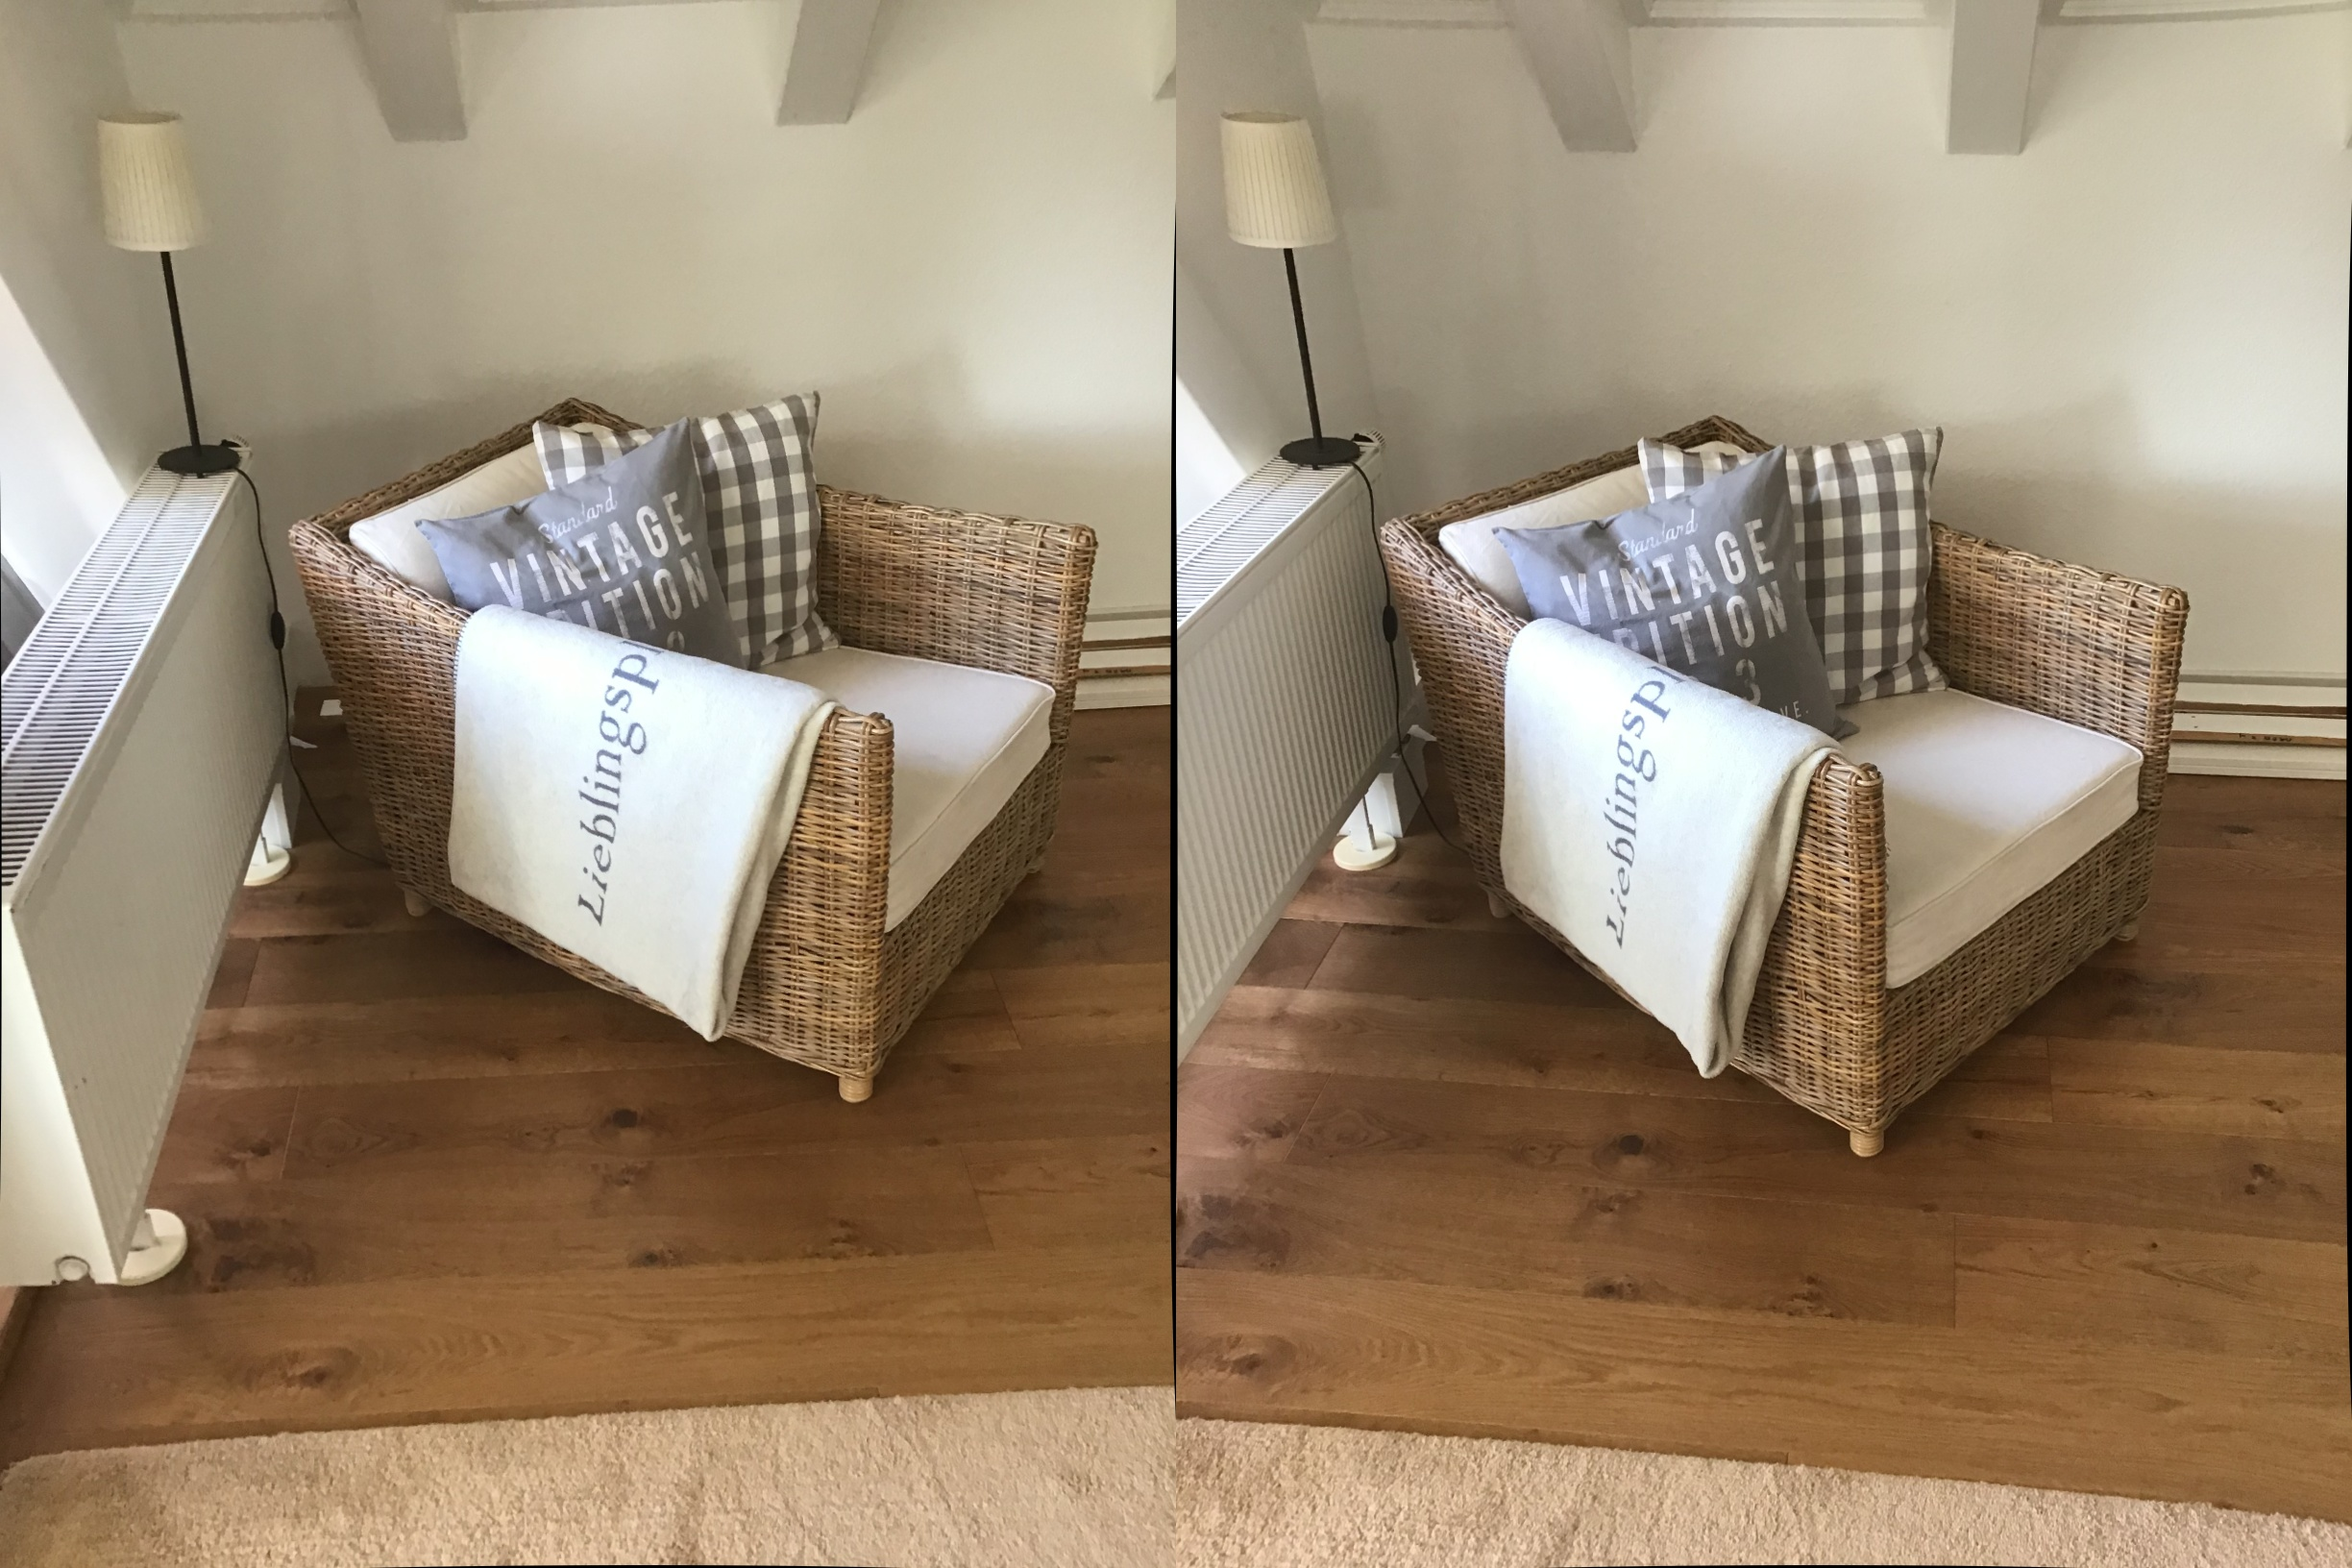
\includegraphics[width=\textwidth]{src/img/chair_first_pair.jpg}
    \caption{Eins von zehn Bildpaaren zum Rekonstruieren des Sessels.}
    \label{fig:chair-first-pair}
\end{figure}

\begin{figure}
    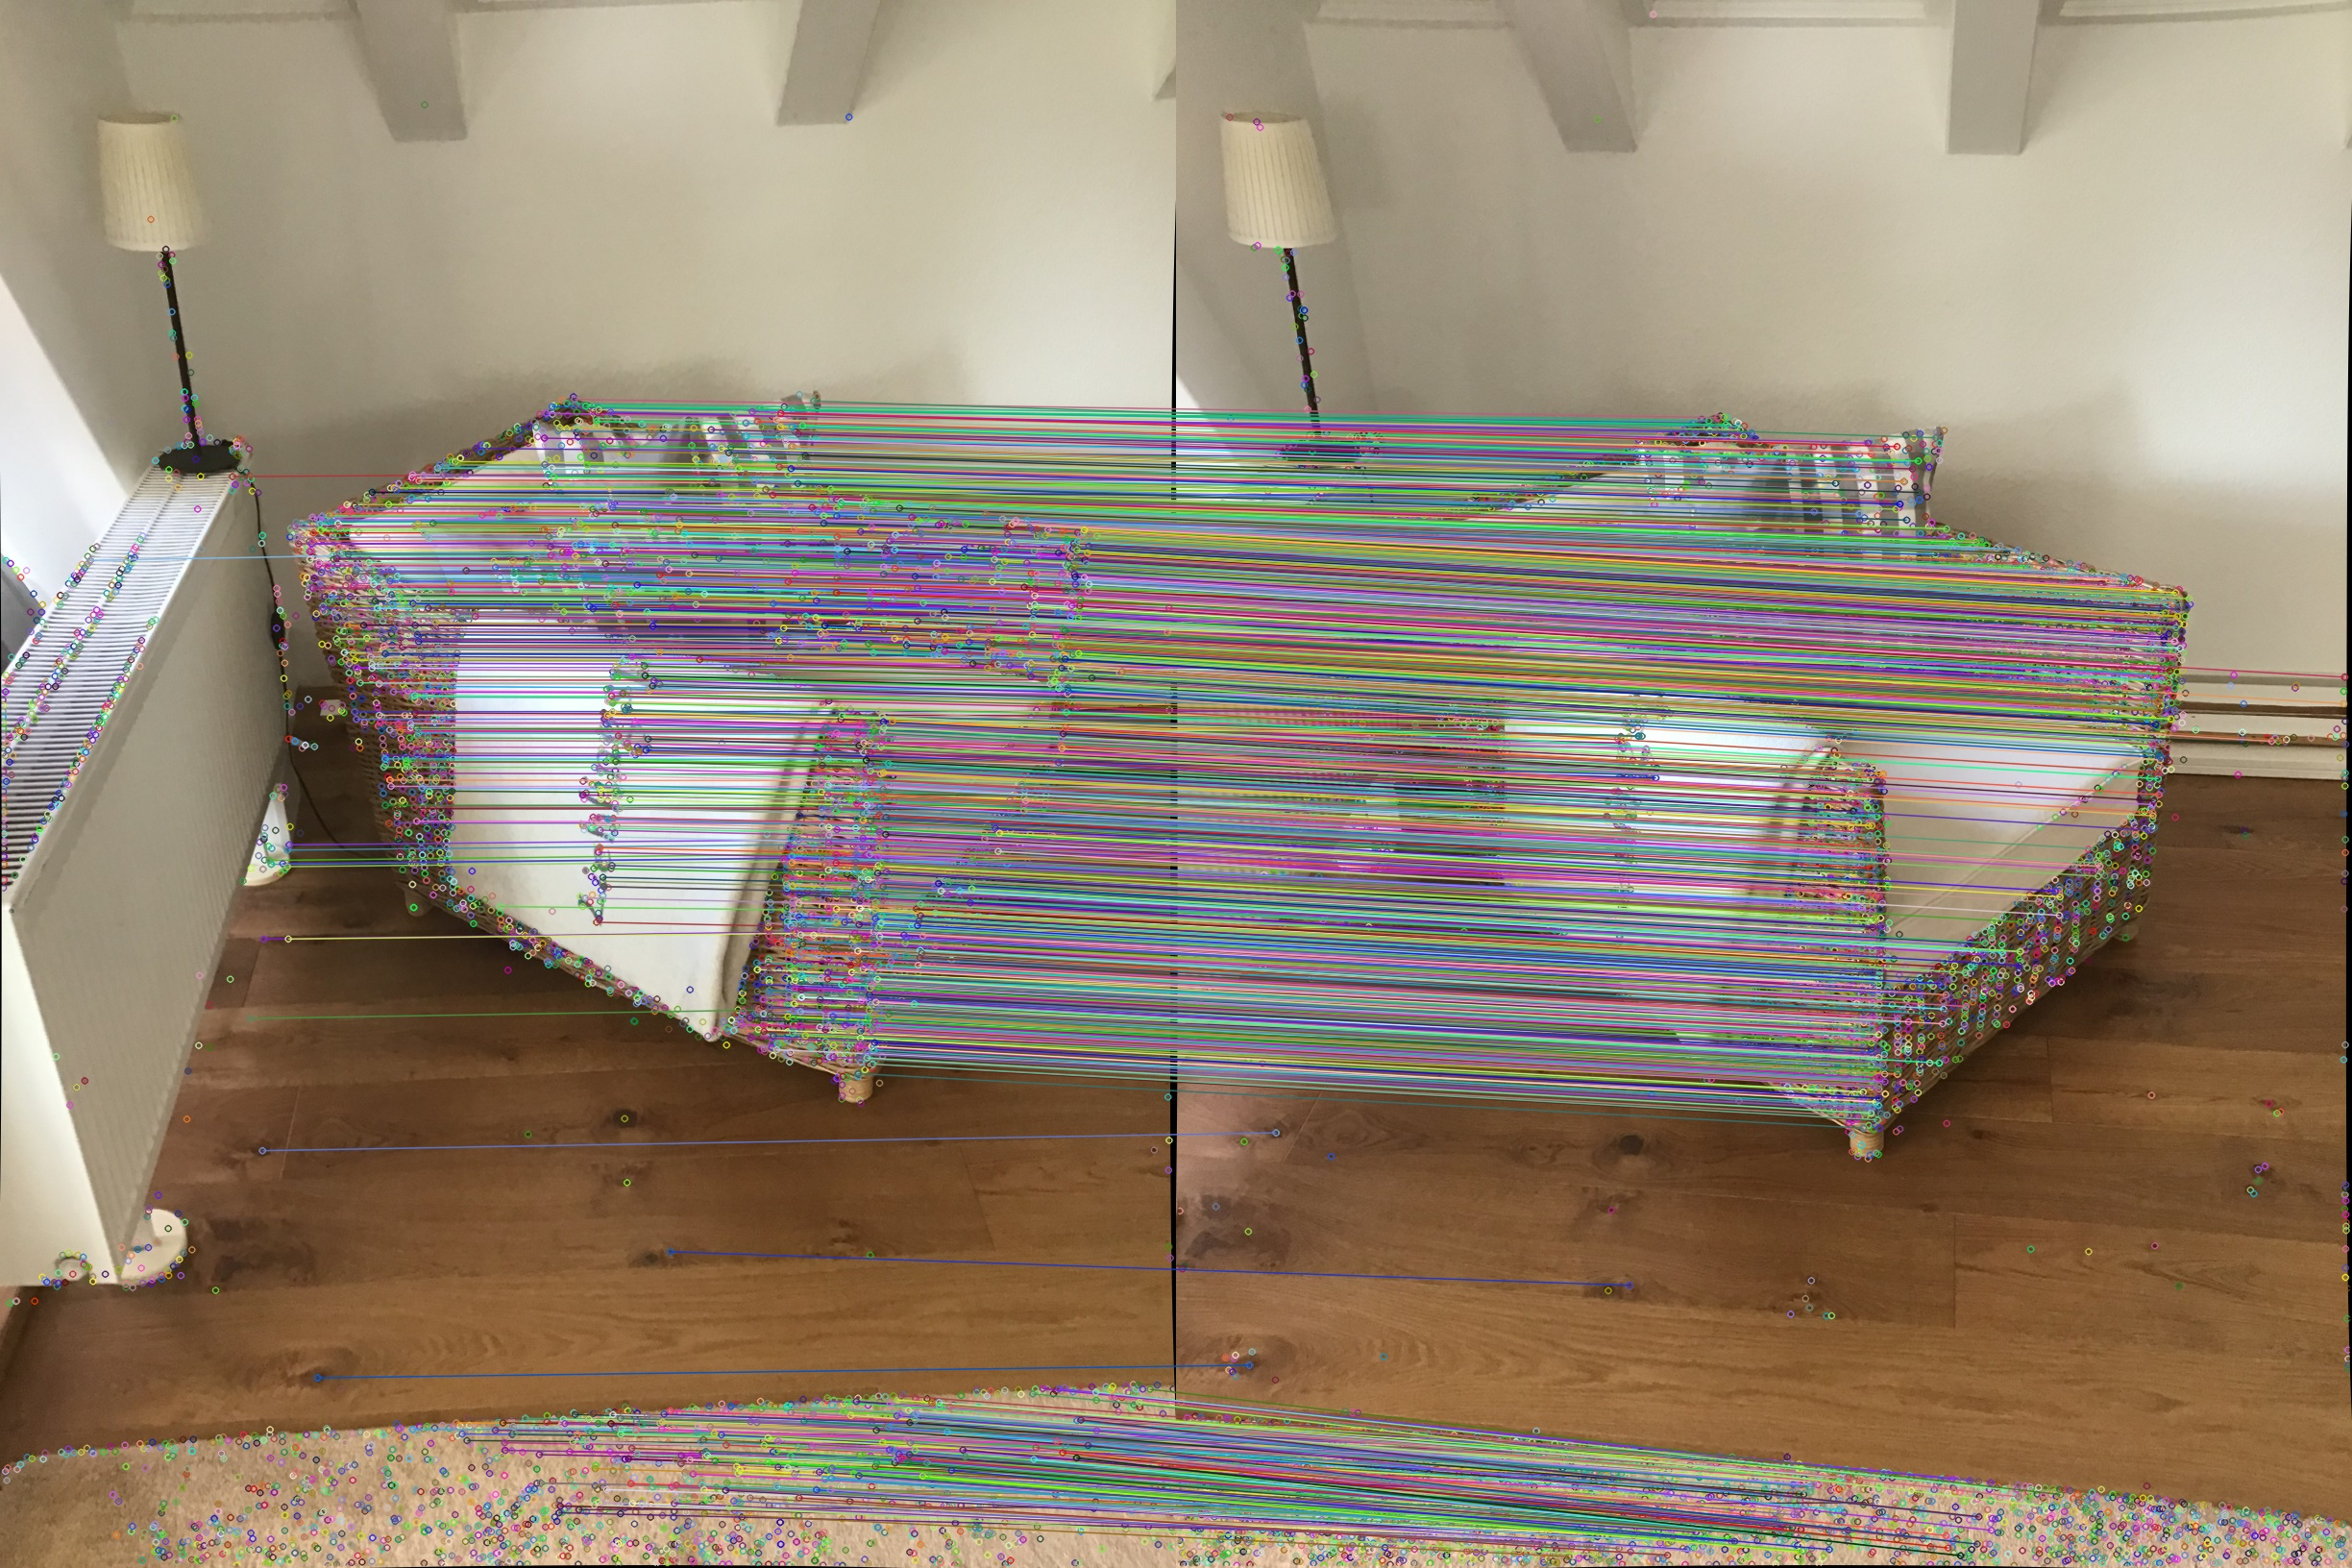
\includegraphics[width=\textwidth]{src/img/chair_first_pair_with_matches.jpg}
    \caption{Bildpaar des Sessels mit Keypoints und Matches.}
    \label{fig:chair-first-pair-with-matches}
\end{figure}

\begin{figure}
    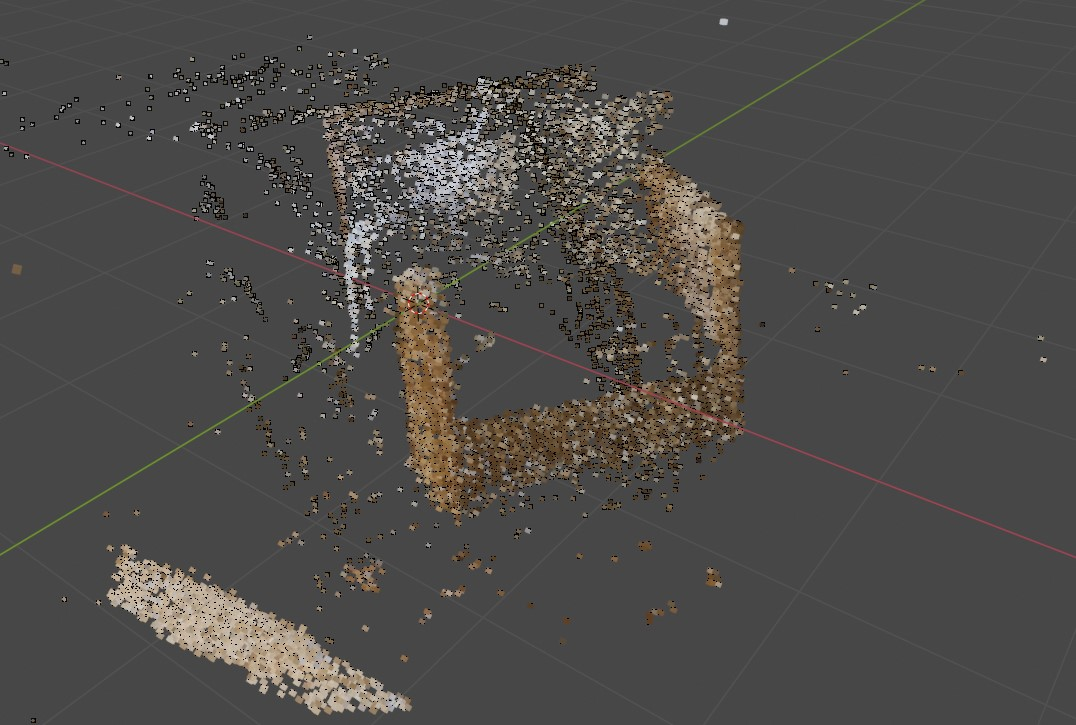
\includegraphics[width=\textwidth]{src/img/chair_model.jpg}
    \caption{Die rekonstruierten Bildpunkte des Sessels in Blender. Das Modell wurde um -119 Grad um die X gedreht, sowie um -4.8 Meter in Y und 2.7 Meter in Z Richtung verschoben.}
    \label{fig:chair-model}
\end{figure}

\begin{figure}
    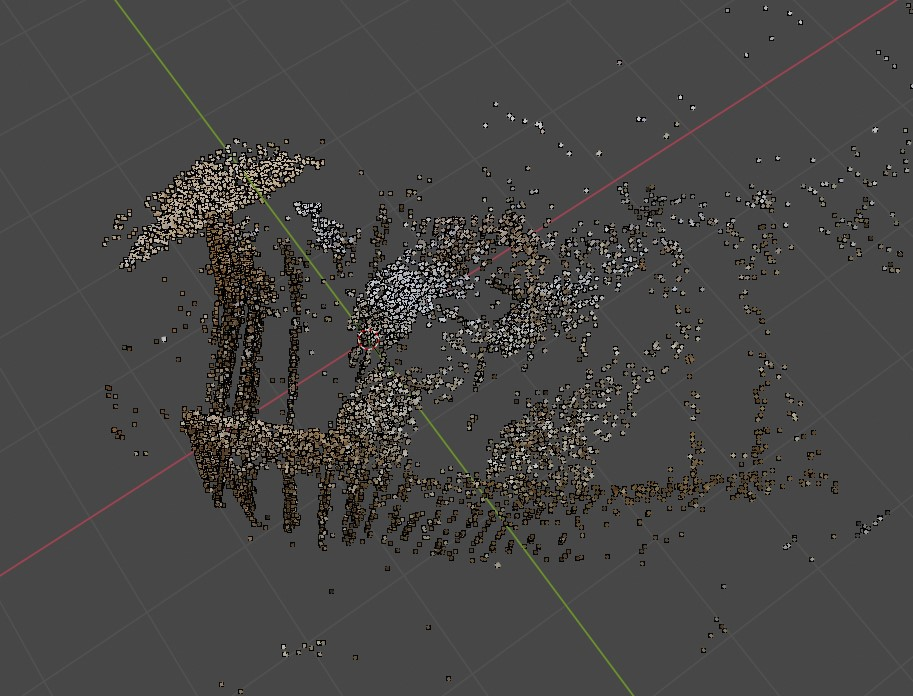
\includegraphics[width=\textwidth]{src/img/chair_model_2.jpg}
    \caption{Das Sessel Modell in einem anderem Blickwinkel}
    \label{fig:chair-model}
\end{figure}


\section{Fall 2: Hase mit Blumen}
\section{Fall 3: Hund}
